% 115-1 ECD HW3 Report  —  compile with XeLaTeX
\documentclass[11pt,a4paper]{article}
\usepackage[margin=2.2cm]{geometry}
\usepackage{fontspec}
% 字型：有 Noto CJK 就用 Noto，否則改用 Windows 內建的微軟正黑體
\IfFontExistsTF{Noto Serif CJK TC}{%
  \setmainfont{Noto Serif CJK TC}
  \setsansfont{Noto Sans CJK TC}
}{%
  \setmainfont{Microsoft JhengHei}
  \setsansfont{Microsoft JhengHei}
}
\XeTeXlinebreaklocale "zh"
\XeTeXlinebreakskip = 0pt plus 1pt
\usepackage{amsmath}
\usepackage{graphicx}
\usepackage{float}
\usepackage{booktabs}
\usepackage{caption}
\usepackage{subcaption}
\usepackage[hidelinks]{hyperref}
\captionsetup{font=small,labelfont=bf}
\renewcommand{\figurename}{Fig.}
\renewcommand{\tablename}{Table}
\linespread{1.25}
\setlength{\parindent}{0pt}
\setlength{\parskip}{6pt}

\newcommand{\Iout}{I_{out}}
\newcommand{\Iref}{I_{REF}}
\newcommand{\Vout}{V_{out}}
\newcommand{\ratio}{\Iout/\Iref}

\title{\textbf{115-1 ECD HW3}}
\author{許楷翊\quad B13901040}
\date{}

\begin{document}
%\maketitle
\vspace{-1.5em}

\section*{115-1 ECD HW3 模擬環境與元件}
\begin{itemize}\setlength{\itemsep}{0pt}
  \item Schematic 中的 instance 名稱與題目圖中的編號不同，對照如 Table~\ref{tab:map}。
\end{itemize}

\begin{table}[H]
  \centering
  \caption{題目元件編號與 schematic instance 名稱對照}
  \label{tab:map}
  \begin{tabular}{lcccc}
    \toprule
              & 題目 $M_1$（參考端） & 題目 $M_2$（輸出端） & 題目 $M_3$ & 題目 $M_4$ \\
    \midrule
    Problem 1 & M2            & M0            & --       & --       \\
    Problem 2 & M2            & M0            & M3       & M1       \\
    Problem 3 & M1            & M0（$m=4$）     & --       & --       \\
    \bottomrule
  \end{tabular}
\end{table}

%=====================================================================
\section{Basic Current Mirror（Fig.~1）}

$\Iref=20\,\mu$A（理想電流源），$M_1=M_2$，分別以 $L=20$\,nm 與 $L=240$\,nm 模擬。
Fig.~\ref{fig:p1sch} 為兩種設計的 schematic（標示元件尺寸與 DC node voltage）。

\begin{figure}[H]
  \centering
  \begin{subfigure}{\textwidth}\centering
    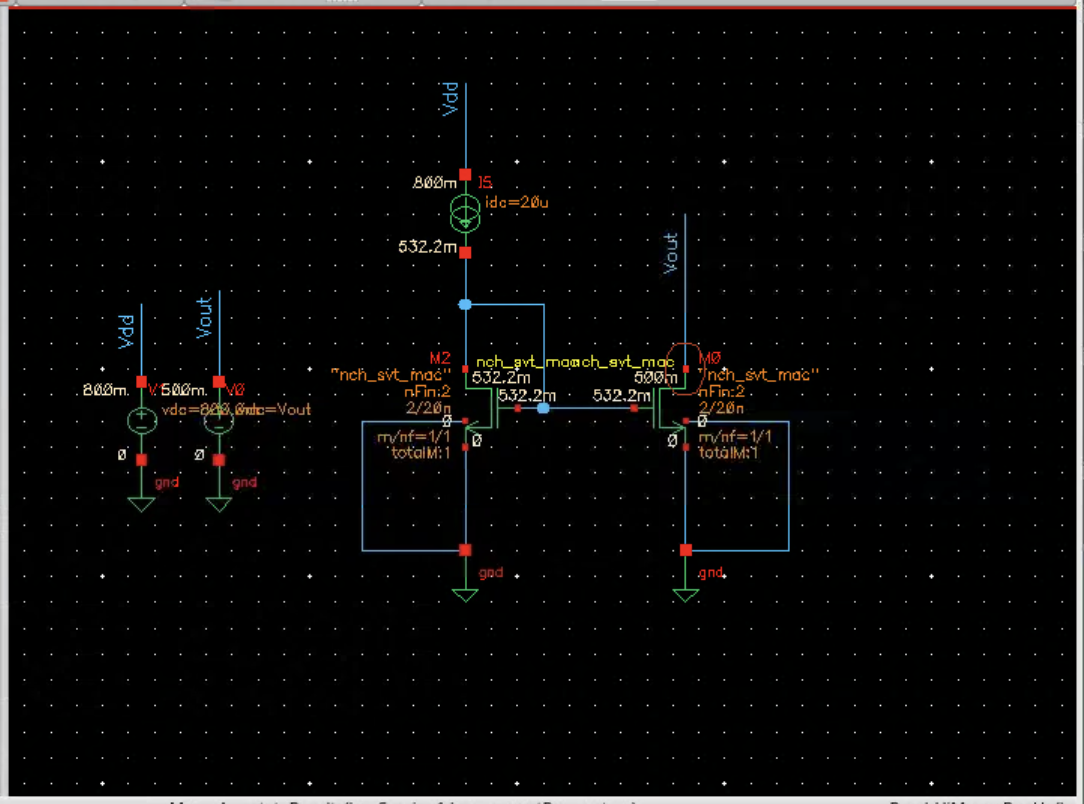
\includegraphics[width=0.78\linewidth,trim=29.5bp 89.0bp 121.0bp 29.0bp,clip]{P1_L=20n_schematic.png}
    \caption{$L=20$\,nm}
  \end{subfigure}\\[6pt]
\end{figure}

\begin{figure}[H]
  \begin{subfigure}{\textwidth}\centering
    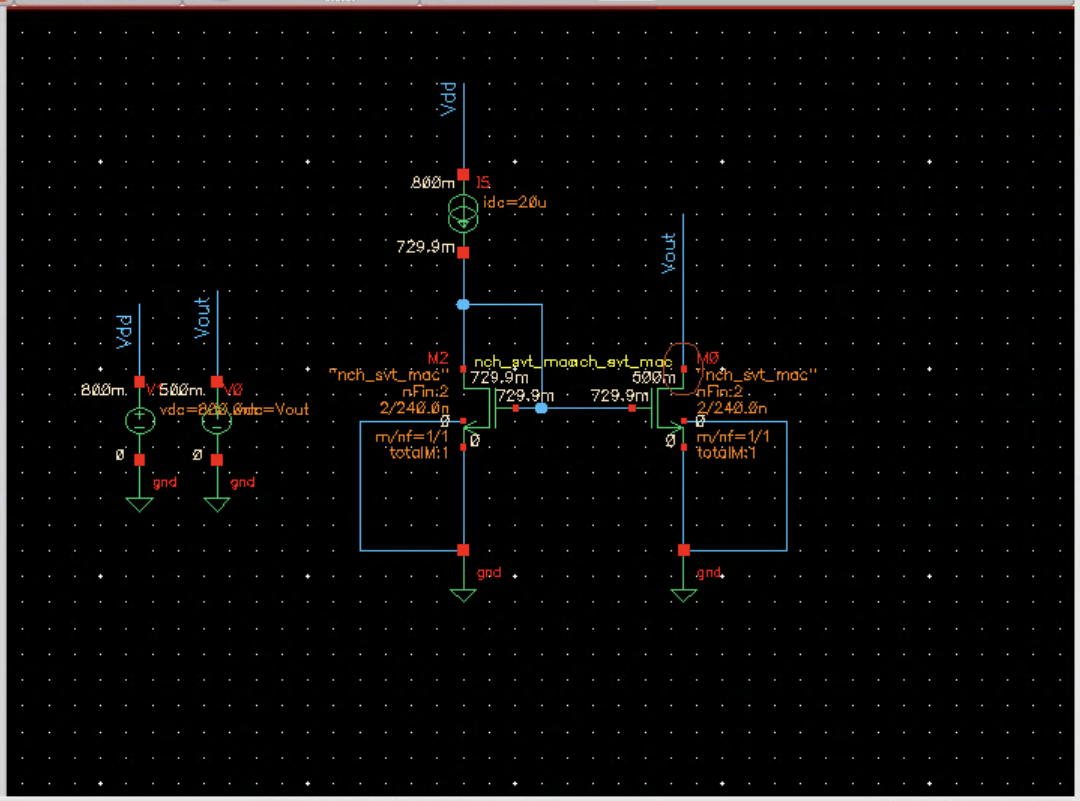
\includegraphics[width=0.78\linewidth,trim=28.5bp 87.5bp 120.0bp 29.0bp,clip]{P1_L=240n_schematic.png}
    \caption{$L=240$\,nm}
  \end{subfigure}
  \caption{Problem 1 schematic（nFin $=2$，$m/nf=1/1$）。閘極節點電壓即為 $V_{GS1}$。}
  \label{fig:p1sch}
\end{figure}

\subsection*{(a) $\ratio$ vs.\ $\Vout$}
$\Vout$ 由 0 掃到 0.8\,V，輸出運算式為 $\Iout/\Iref$，結果如 Fig.~\ref{fig:p1ratio}。

\begin{figure}[H]
  \centering
  \begin{subfigure}{\textwidth}\centering
    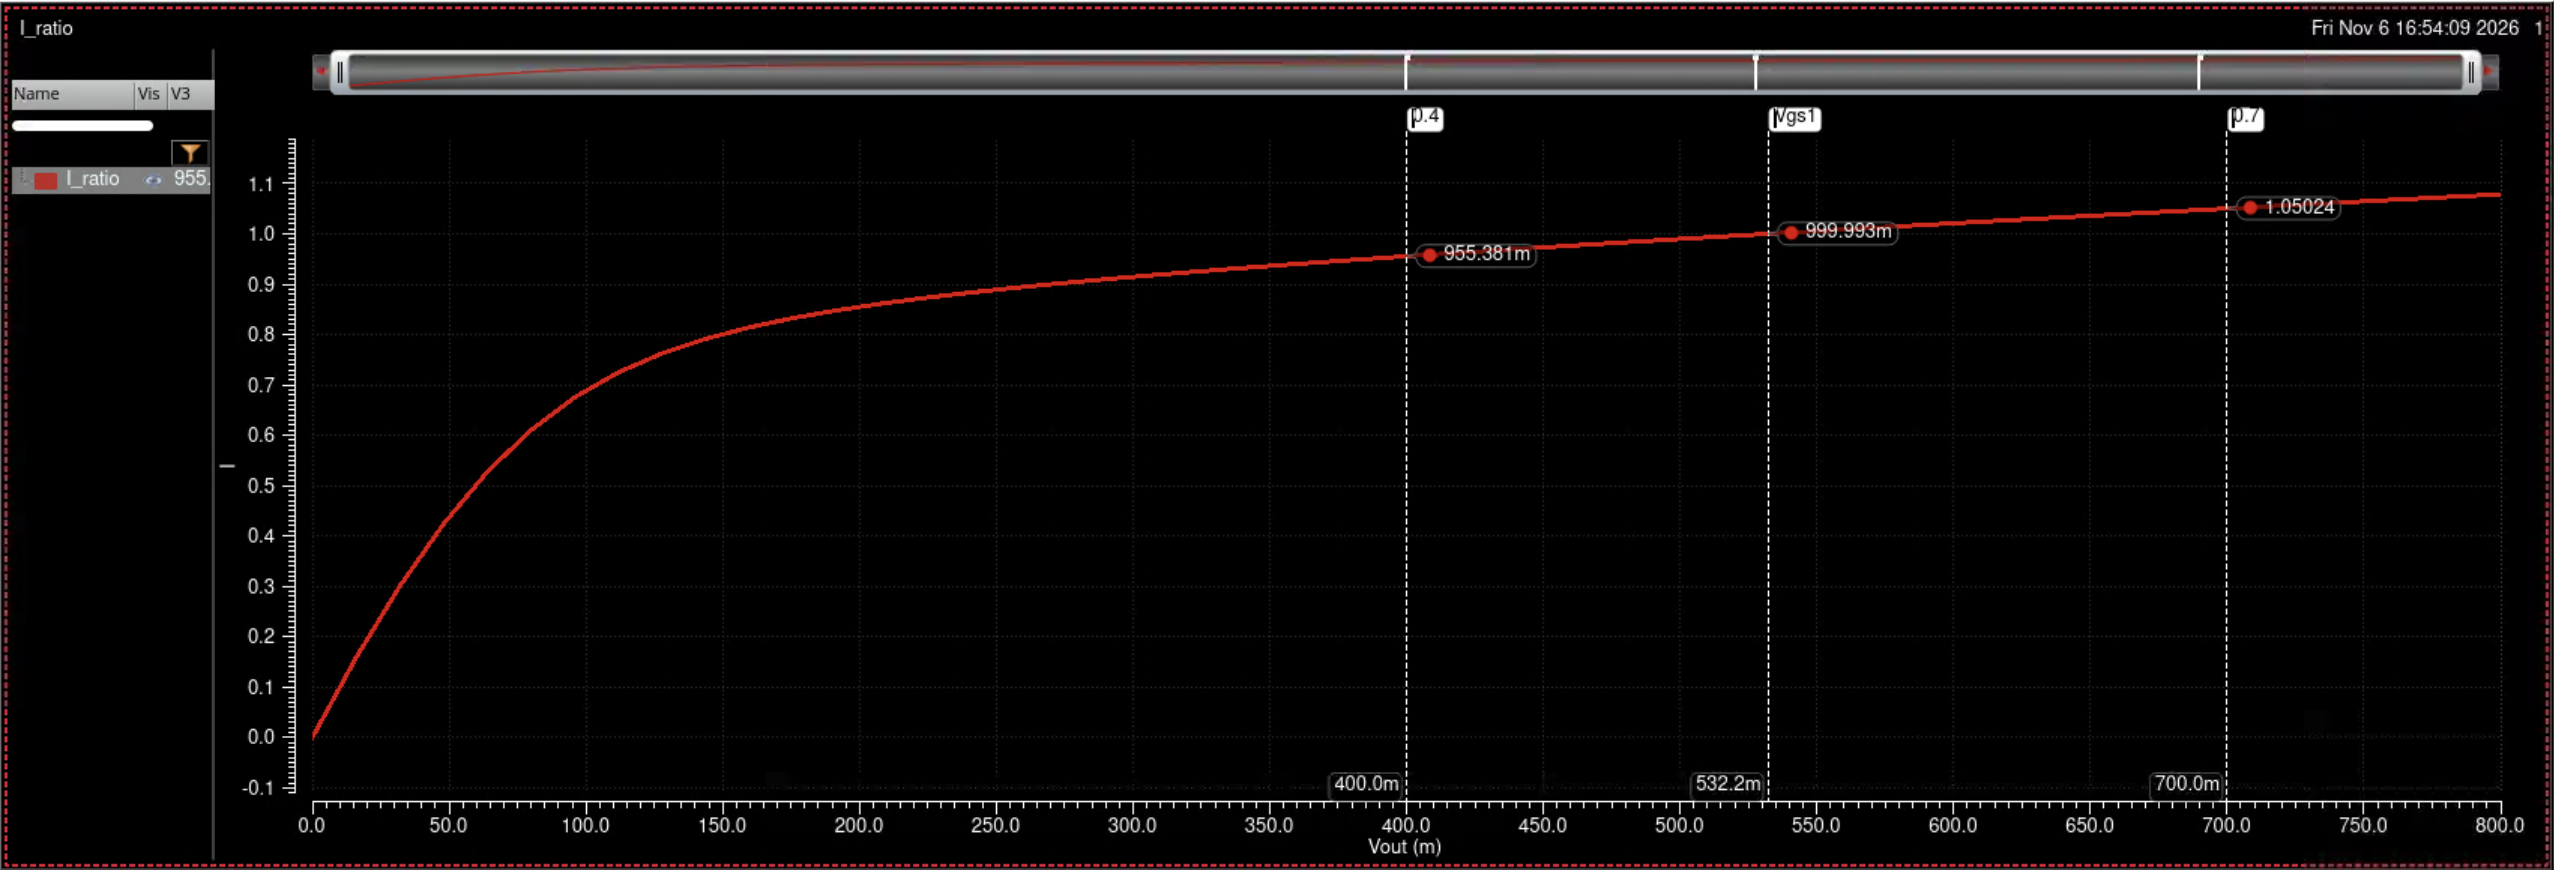
\includegraphics[width=\linewidth]{P1_L=20n_Iratio.png}
    \\[3pt]
    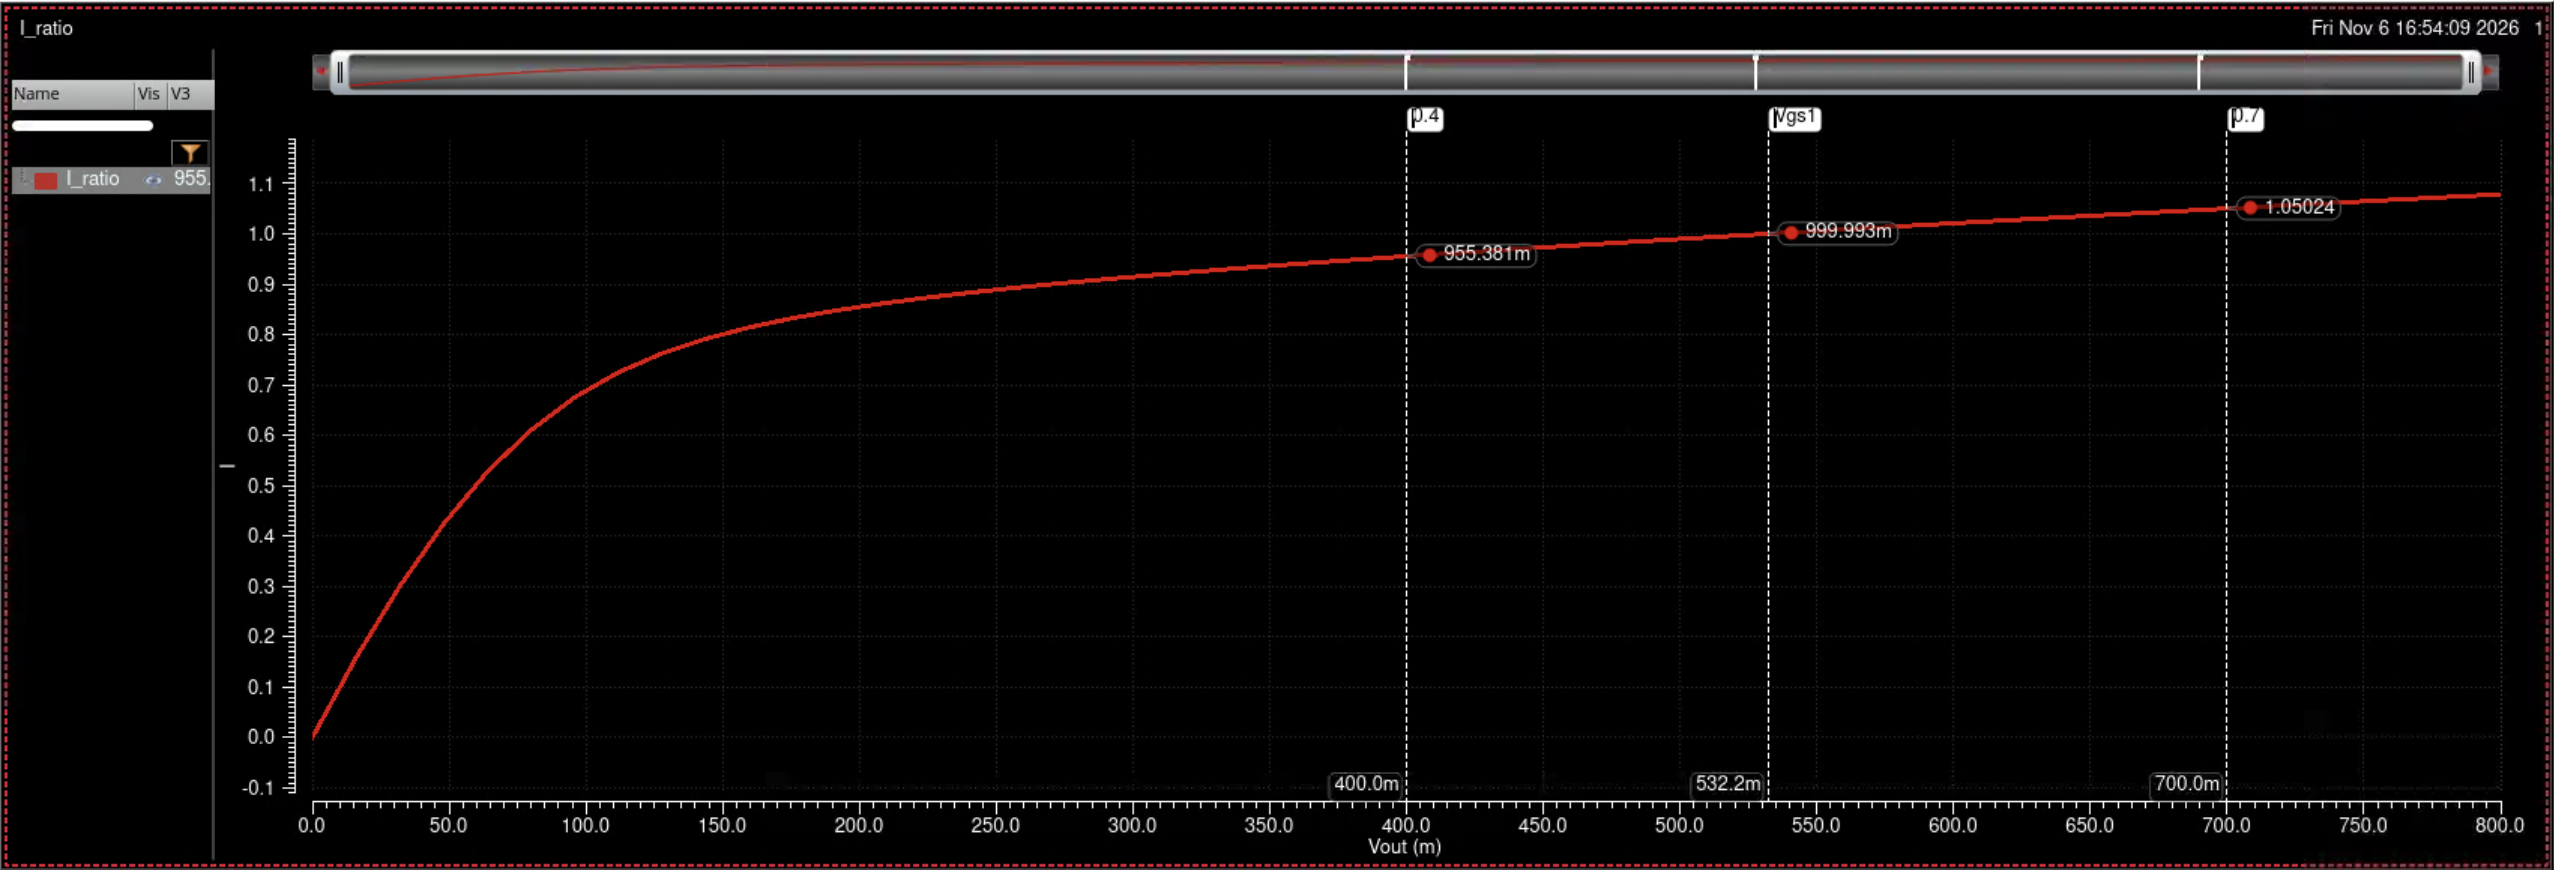
\includegraphics[width=0.9\linewidth,trim=665.0bp 285.0bp 4.5bp 47.5bp,clip]{P1_L=20n_Iratio.png}
    \caption{$L=20$\,nm}
  \end{subfigure}\\[4pt]
\end{figure}

\begin{figure}[H]
  \begin{subfigure}{\textwidth}\centering
    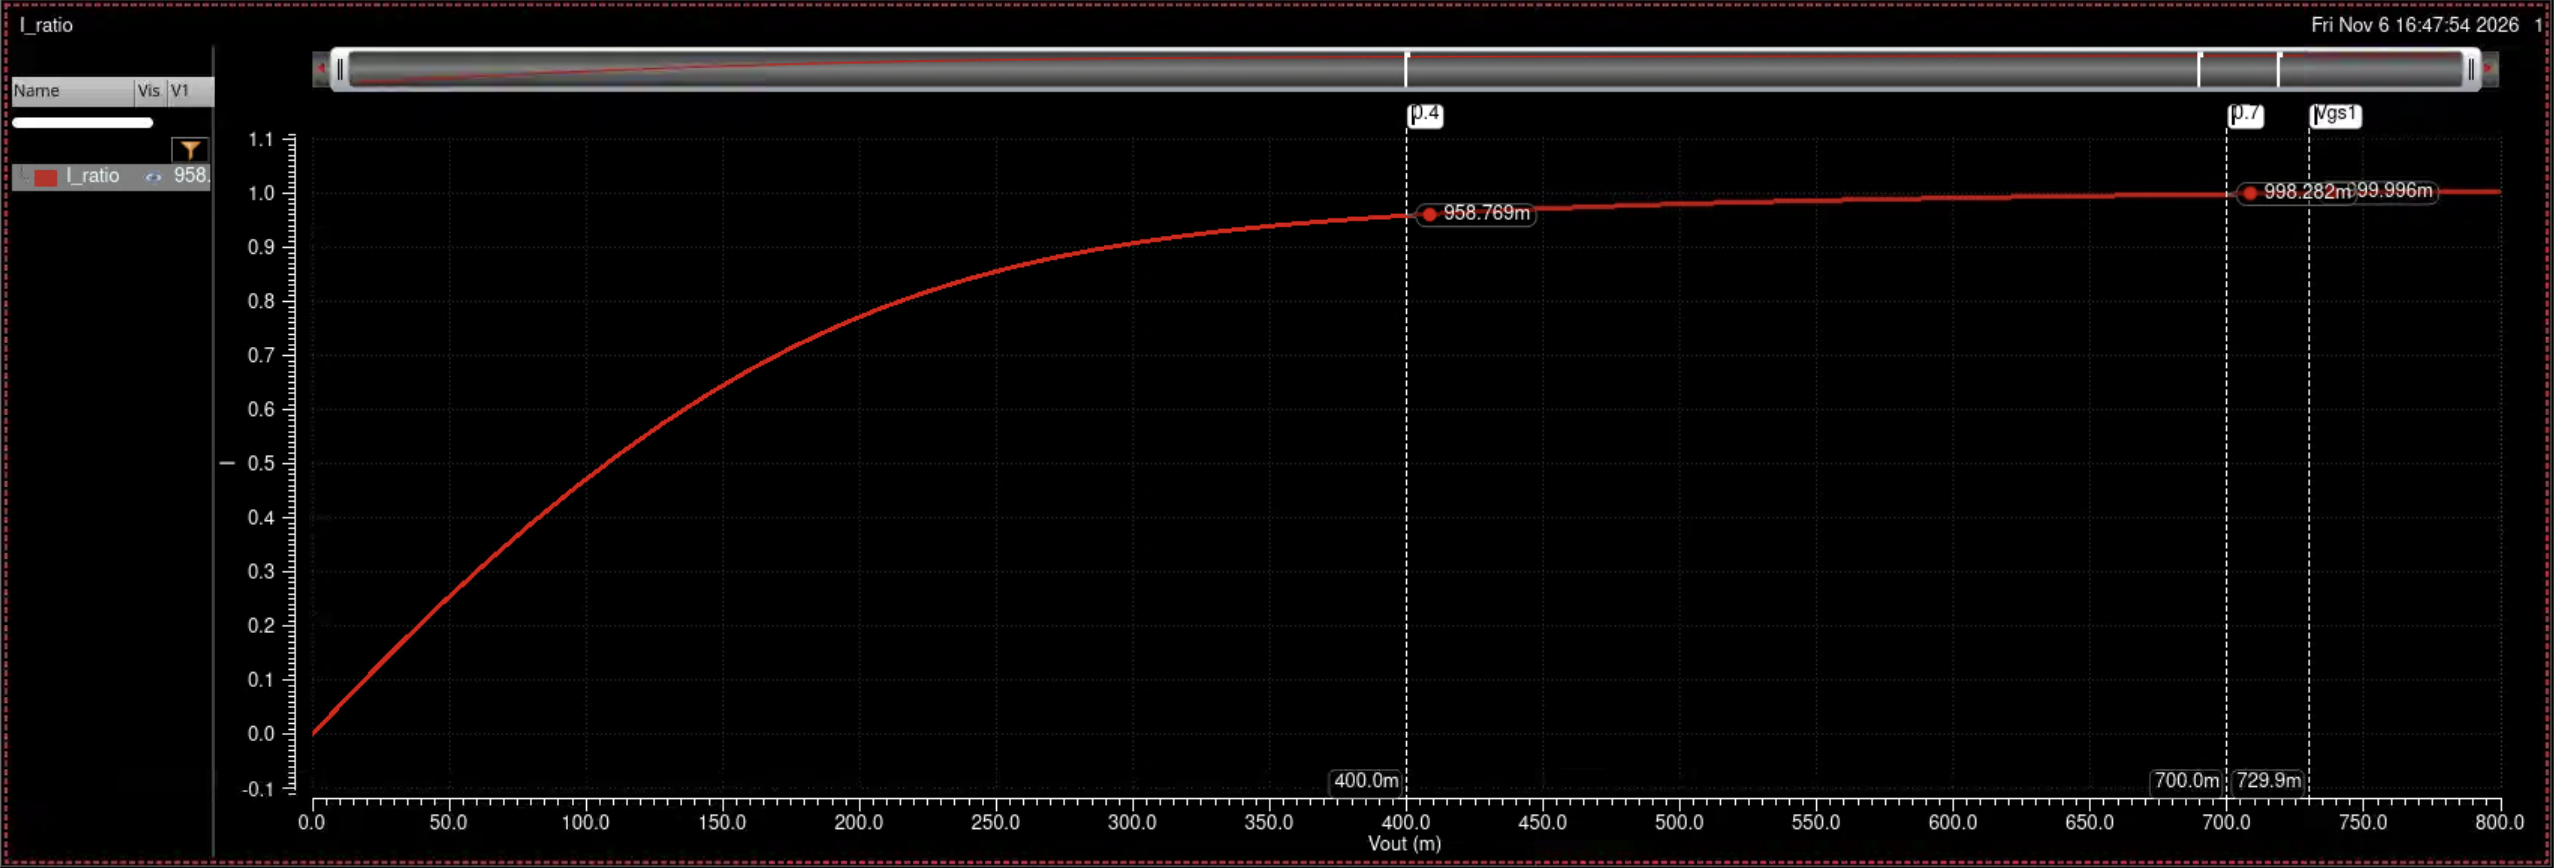
\includegraphics[width=\linewidth]{P1_L=240n_Iratio.png}
    \\[3pt]
    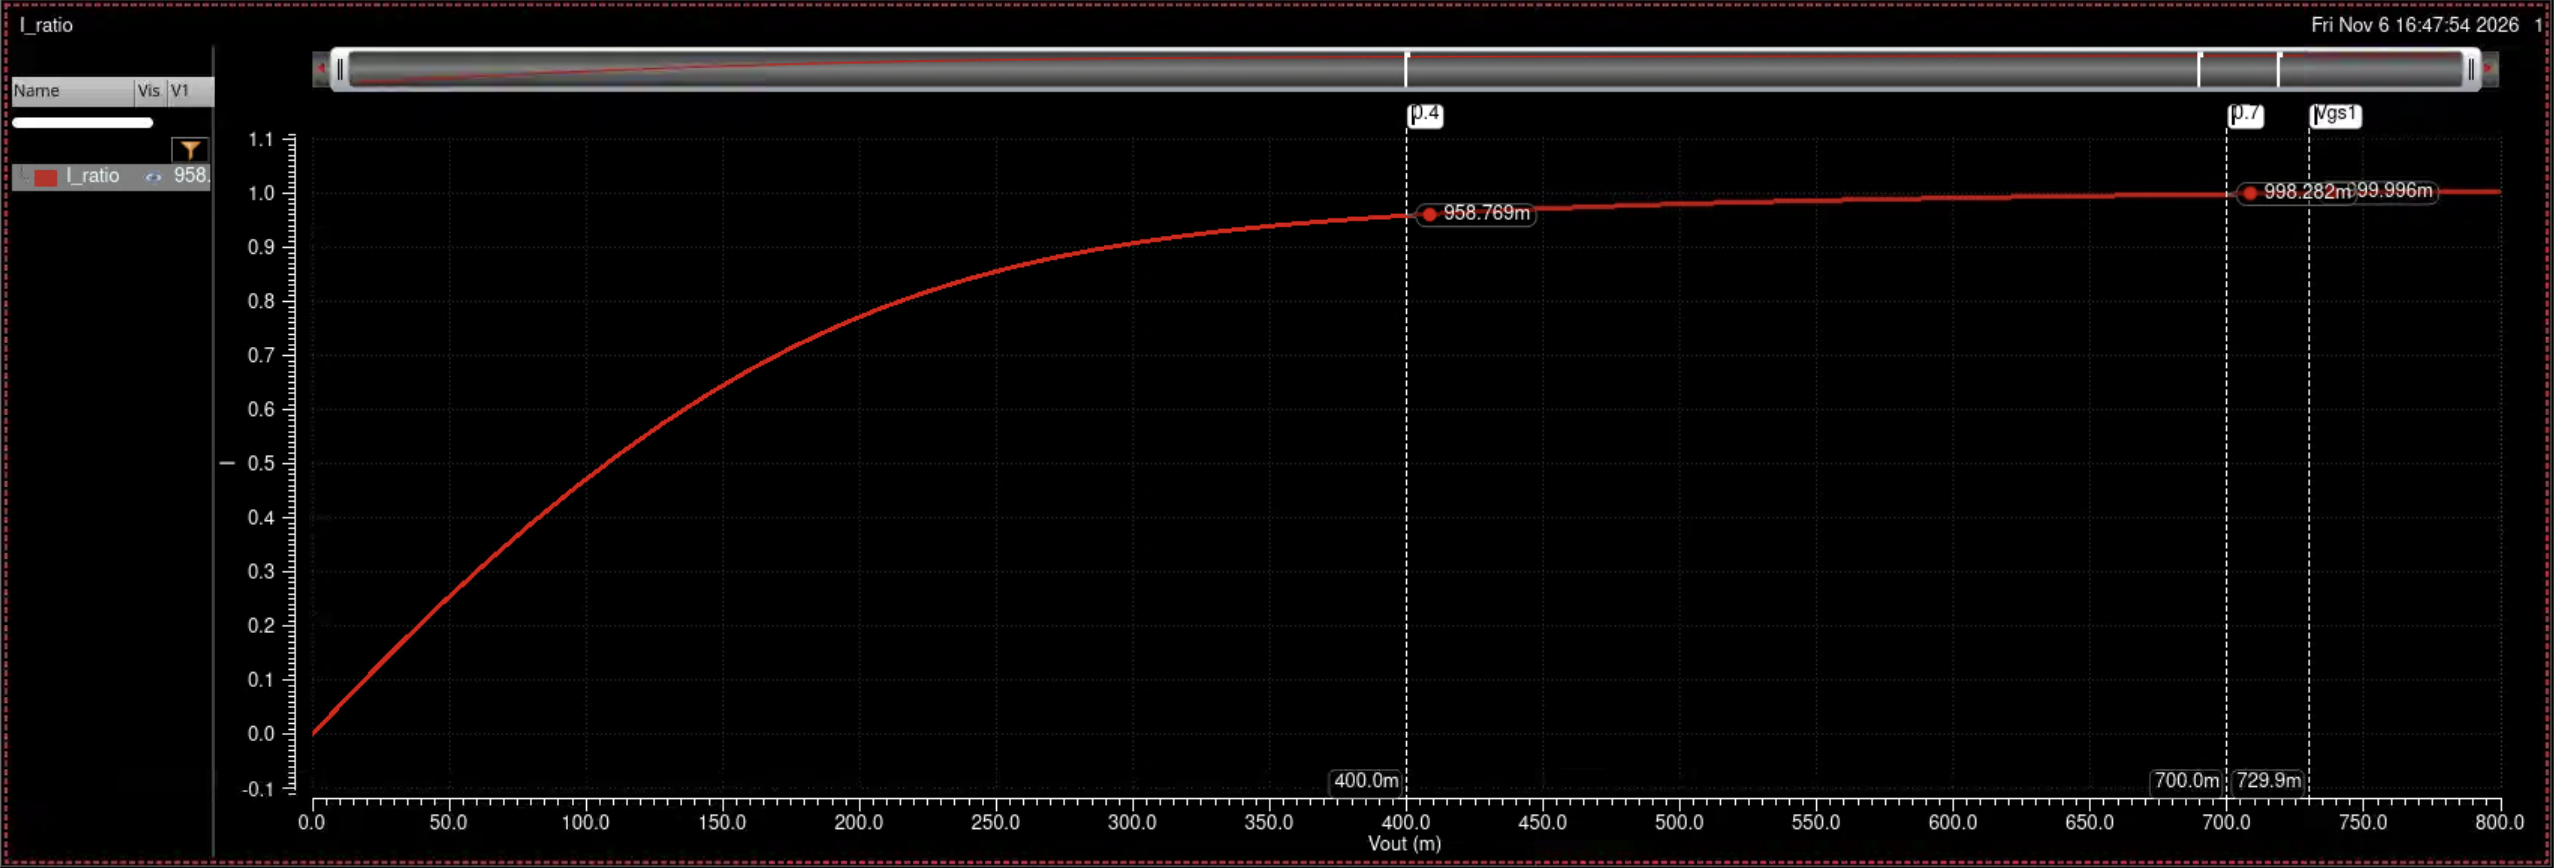
\includegraphics[width=0.9\linewidth,trim=665.0bp 304.0bp 4.5bp 47.5bp,clip]{P1_L=240n_Iratio.png}
    \caption{$L=240$\,nm}
  \end{subfigure}
  \caption{Problem 1：$\ratio$ vs.\ $\Vout$，marker 位於 $\Vout=0.4$\,V、$V_{GS1}$、0.7\,V；每張下方為 marker 區域放大。}
  \label{fig:p1ratio}
\end{figure}

\subsection*{(b) $\Vout=V_{GS1}$ 時的 $\ratio$}
\begin{itemize}\setlength{\itemsep}{0pt}
  \item $L=20$\,nm：$V_{GS1}=532.2$\,mV，$\ratio=0.99999$。
  \item $L=240$\,nm：$V_{GS1}=729.9$\,mV，$\ratio=0.99999$（$=999.996$\,m）。
\end{itemize}
兩者皆 $\approx 1$。原因：$M_1$ 為 diode-connected，$V_{DS1}=V_{GS1}$；
當 $\Vout=V_{GS1}$ 時 $V_{DS2}=V_{DS1}$，兩顆尺寸相同、$V_{GS}$ 相同，
三個條件完全一致，因此 $I_{D2}=I_{D1}$。這是唯一一個 channel-length modulation
不造成誤差的偏壓點，與 $L$ 無關（nominal 模擬不含隨機 mismatch）。

\subsection*{(c) Mismatch $(\Iout-\Iref)/\Iref$}

\begin{table}[H]
  \centering
  \caption{Problem 1 mismatch}
  \label{tab:p1}
  \small
  \begin{tabular}{lcccc}
    \toprule
                & $\ratio$ @ 0.4\,V & mismatch @ 0.4\,V & $\ratio$ @ 0.7\,V & mismatch @ 0.7\,V \\
    \midrule
    $L=20$\,nm  & 0.9554            & $-4.46\%$         & 1.0502            & $+5.02\%$         \\
    $L=240$\,nm & 0.9588            & $-4.12\%$         & 0.9983            & $-0.17\%$         \\
    \bottomrule
  \end{tabular}
\end{table}

\textbf{長通道（$L=240$\,nm）的 mismatch 較小}，在 0.7\,V 時尤其明顯（$0.17\%$ vs.\ $5.02\%$）。

在飽和區，$\ratio \approx (1+\lambda\Vout)/(1+\lambda V_{GS1})$，mismatch 隨 $|\Vout-V_{GS1}|$
與 $\lambda$ 成正比。以 $V_{GS1}$ 與 0.7\,V 兩點反推等效 $\lambda$：
\[
  \lambda_{20\,\mathrm{nm}} \approx 0.36\ \mathrm{V^{-1}},\qquad
  \lambda_{240\,\mathrm{nm}} \approx 0.06\ \mathrm{V^{-1}}.
\]
通道越長，汲極電場對通道的調變（channel-length modulation、DIBL）越弱，
$r_o$ 越大，所以 $\Iout$ 隨 $\Vout$ 的變化越小。兩者比值約 6 倍，小於 $L$ 的比值 12 倍，
代表短通道效應不是單純的 $\lambda\propto 1/L$。

值得注意的是，在 $\Vout=0.4$\,V 時兩者的 mismatch 相近（約 $-4\%$）。原因是長通道元件要流
同樣 20\,$\mu$A 需要較大的 overdrive：$V_{GS1}=729.9$\,mV、$V_{DS,sat}=289.5$\,mV
（短通道只有 104.9\,mV）。$\Vout=0.4$\,V 只略高於 $V_{DS,sat}$，$M_2$ 位於飽和區與三極區的
過渡段，曲線尚未變平；短通道在 0.4\,V 時則已穩定飽和，其 $-4.46\%$ 主要來自 channel-length modulation。
因此長 $L$ 以較小的 $\lambda$ 換得較佳匹配，代價是較大的 $V_{DS,sat}$ 與較小的輸出擺幅（headroom）。

%=====================================================================
\section{Cascode Current Mirror（Fig.~2）}

在 Problem 1 的短通道 mirror（$L=20$\,nm）上疊加 cascode 元件 $M_{3}$、$M_{4}$，
四顆尺寸皆為 nFin $=2$、$L=20$\,nm；$V_b$ 為理想電壓源，$\Iref=20\,\mu$A。
$M_1$、$M_2$ 的閘極接至 $\Iref$ 節點（$M_3$ 的 drain），$M_3$、$M_4$ 的閘極接 $V_b$，
即 low-voltage cascode 架構。Schematic 如 Fig.~\ref{fig:p2sch}。

\begin{figure}[H]
  \centering
  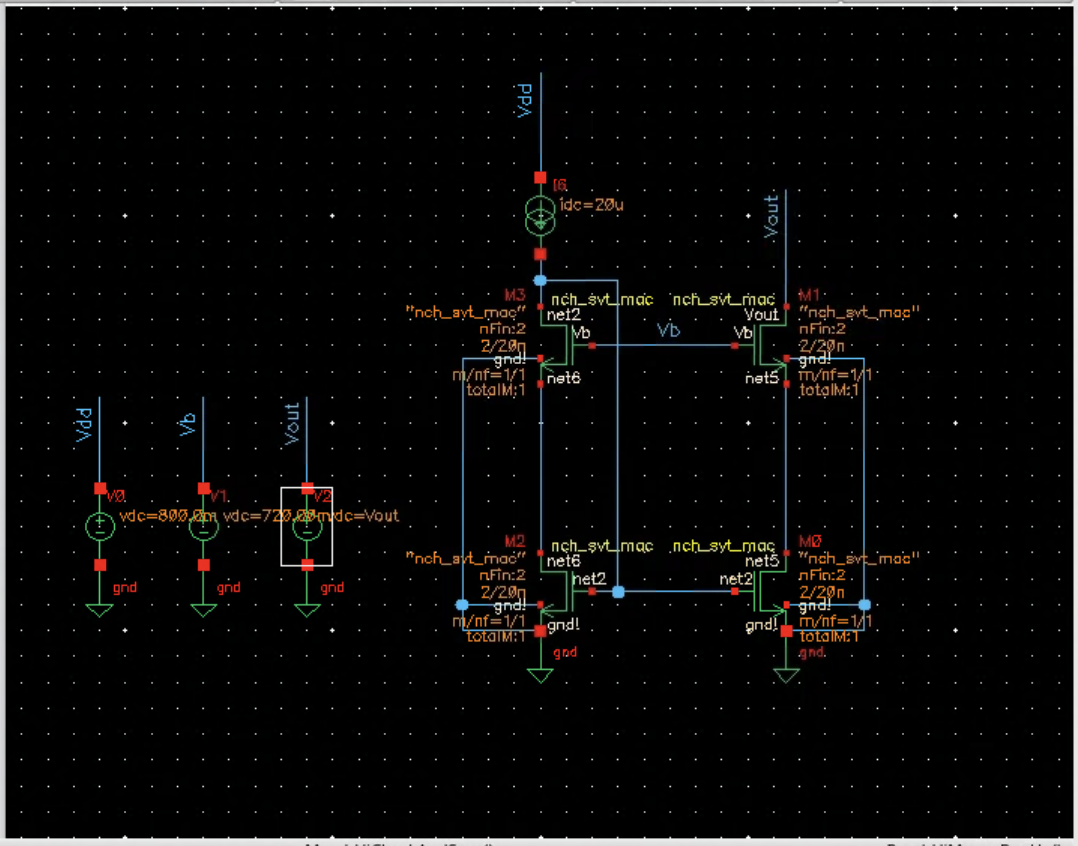
\includegraphics[width=0.85\textwidth,trim=25.5bp 69.5bp 70.0bp 29.5bp,clip]{P2_schematic.png}
  \caption{Problem 2 schematic（四顆皆為 nFin $=2$、$L=20$\,nm，$V_b=720$\,mV）。}
  \label{fig:p2sch}
\end{figure}

\subsection*{(a) 選擇 $V_b$}
令 $M_1$/$M_3$ 間節點為 $X$，$M_2$/$M_4$ 間節點為 $Y$。$\Iref$ 節點電壓為 $V_{GS1}$，$V_X=V_b-V_{GS3}$。
\begin{align*}
  M_1\ \text{飽和：}\quad & V_X \ge V_{DS,sat1}
  \;\Rightarrow\; V_b \ge V_{GS3}+V_{DS,sat1}      \\
  M_3\ \text{飽和：}\quad & V_{GS1} \ge V_b - V_{TH3}
  \;\Rightarrow\; V_b \le V_{GS1}+V_{TH3}
\end{align*}
$M_2$、$M_4$ 與 $M_1$、$M_3$ 對稱：$M_4$ 飽和時 $V_Y\approx V_X$，故 $V_{DS2}\approx V_{DS1}$；
另外 $M_4$ 飽和需要 $\Vout \ge V_b - V_{TH4}$。

初估時沿用 Problem 1 短通道的 $V_{GS}\approx532$\,mV、$V_{TH}\approx373$\,mV，
得到 $V_b$ 約 0.69--0.8\,V（上限 $V_{GS1}+V_{TH}\approx0.9$\,V 超過 $V_{DD}$，故受 $V_{DD}$ 限制），
取 $V_b=0.72$\,V。

以 $\Vout=0.5$\,V 標註工作點（Fig.~\ref{fig:p2sat}、Table~\ref{tab:p2sat}）驗證：

\begin{figure}[H]
  \centering
  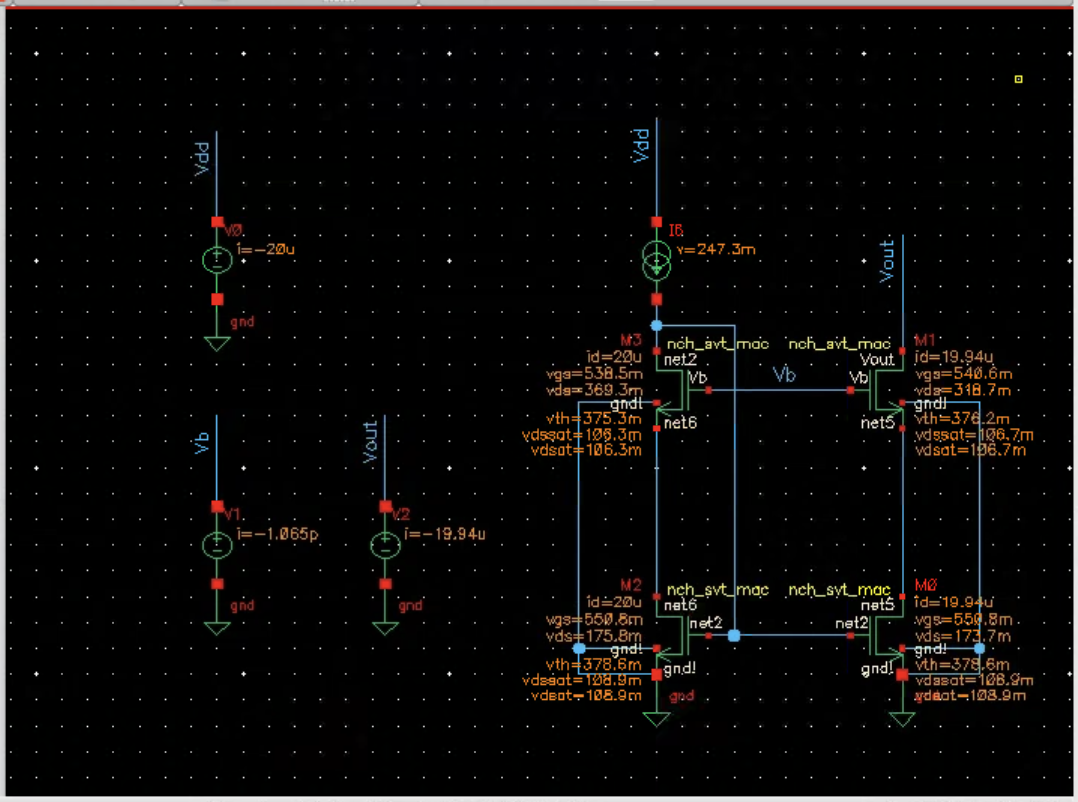
\includegraphics[width=0.85\textwidth,trim=85.0bp 27.0bp 10.5bp 25.0bp,clip]{P2_a_examineSat.png}
  \caption{Problem 2 DC operating point（$V_b=0.72$\,V，$\Vout=0.5$\,V）。}
  \label{fig:p2sat}
\end{figure}

\begin{table}[H]
  \centering
  \caption{Problem 2 工作點（$\Vout=0.5$\,V）}
  \label{tab:p2sat}
  \small
  \begin{tabular}{lccccccc}
    \toprule
    題目元件  & instance & $I_D$         & $V_{GS}$  & $V_{TH}$  & $V_{DS}$  & $V_{DS,sat}$ & $V_{DS}-V_{DS,sat}$ \\
    \midrule
    $M_1$ & M2       & 20.00\,$\mu$A & 550.8\,mV & 378.6\,mV & 175.8\,mV & 108.9\,mV    & $+66.9$\,mV         \\
    $M_2$ & M0       & 19.94\,$\mu$A & 550.8\,mV & 378.6\,mV & 173.7\,mV & 108.9\,mV    & $+64.8$\,mV         \\
    $M_3$ & M3       & 20.00\,$\mu$A & 538.5\,mV & 375.3\,mV & 369.3\,mV & 106.3\,mV    & $+263.0$\,mV        \\
    $M_4$ & M1       & 19.94\,$\mu$A & 540.6\,mV & 376.2\,mV & 318.7\,mV & 106.7\,mV    & $+212.0$\,mV        \\
    \bottomrule
  \end{tabular}
\end{table}

四顆皆滿足 $V_{DS}>V_{DS,sat}$，\textbf{全部位於飽和區}，$V_b=0.72$\,V 可用。
且 $V_{DS1}=175.8$\,mV 與 $V_{DS2}=173.7$\,mV 僅差約 2\,mV，顯示 cascode 使 $V_Y\approx V_X$。

修正：在 cascode 中 $M_1$ 的 $V_{DS}$ 只有約 176\,mV（Problem 1 為 532\,mV），
受 channel-length modulation／DIBL 影響，要流同樣 20\,$\mu$A 需要較大的 $V_{GS1}=550.8$\,mV。
以實際工作點重算 $V_b$ 範圍：
\[
  \underbrace{538.5+108.9}_{V_{GS3}+V_{DS,sat1}}\approx 0.65\ \mathrm{V}
  \;\le\; V_b \;\le\;
  \min\!\big(\underbrace{550.8+375.3}_{V_{GS1}+V_{TH3}}\approx0.93\ \mathrm{V},\ V_{DD}\big)=0.8\ \mathrm{V}.
\]
若改以平方律的 $V_{GS1}-V_{TH1}\approx172$\,mV 作為飽和邊界，下限約 0.71\,V，0.72\,V 幾乎貼著下限；
本報告以模擬器的 $V_{DS,sat}$ 作為飽和判準，$V_b=0.72$\,V 保有約 65\,mV 餘裕。
$V_b$ 越大 $M_1$ 餘裕越多，但 $M_4$ 所需的最低 $\Vout\ (\approx V_b-V_{TH4}\approx0.34$\,V$)$ 也越高，故取靠近下限的值。

\subsection*{(b) $\ratio$ vs.\ $\Vout$（0.1--0.8\,V）}

\begin{figure}[H]
  \centering
  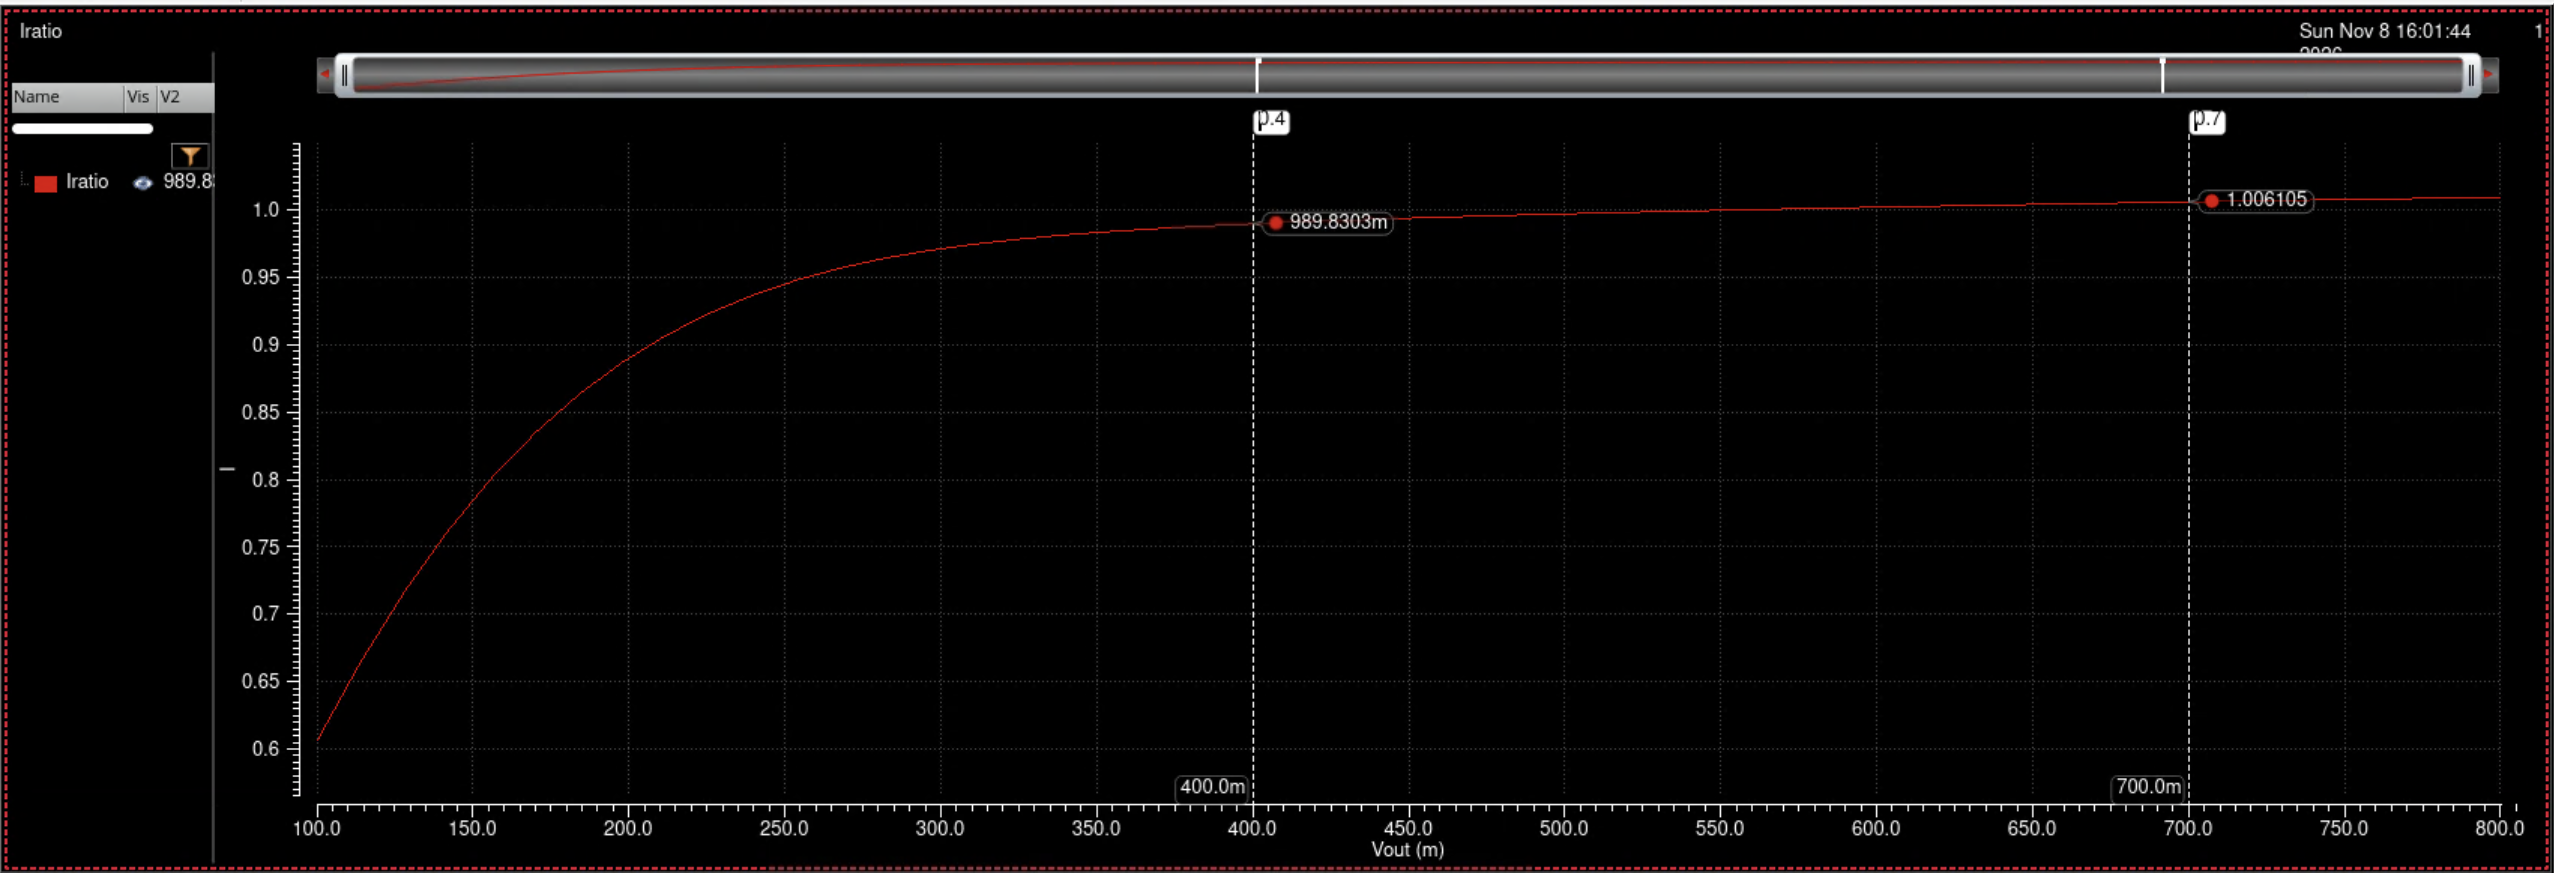
\includegraphics[width=\textwidth]{P2_Iratio.png}
  \\[3pt]
  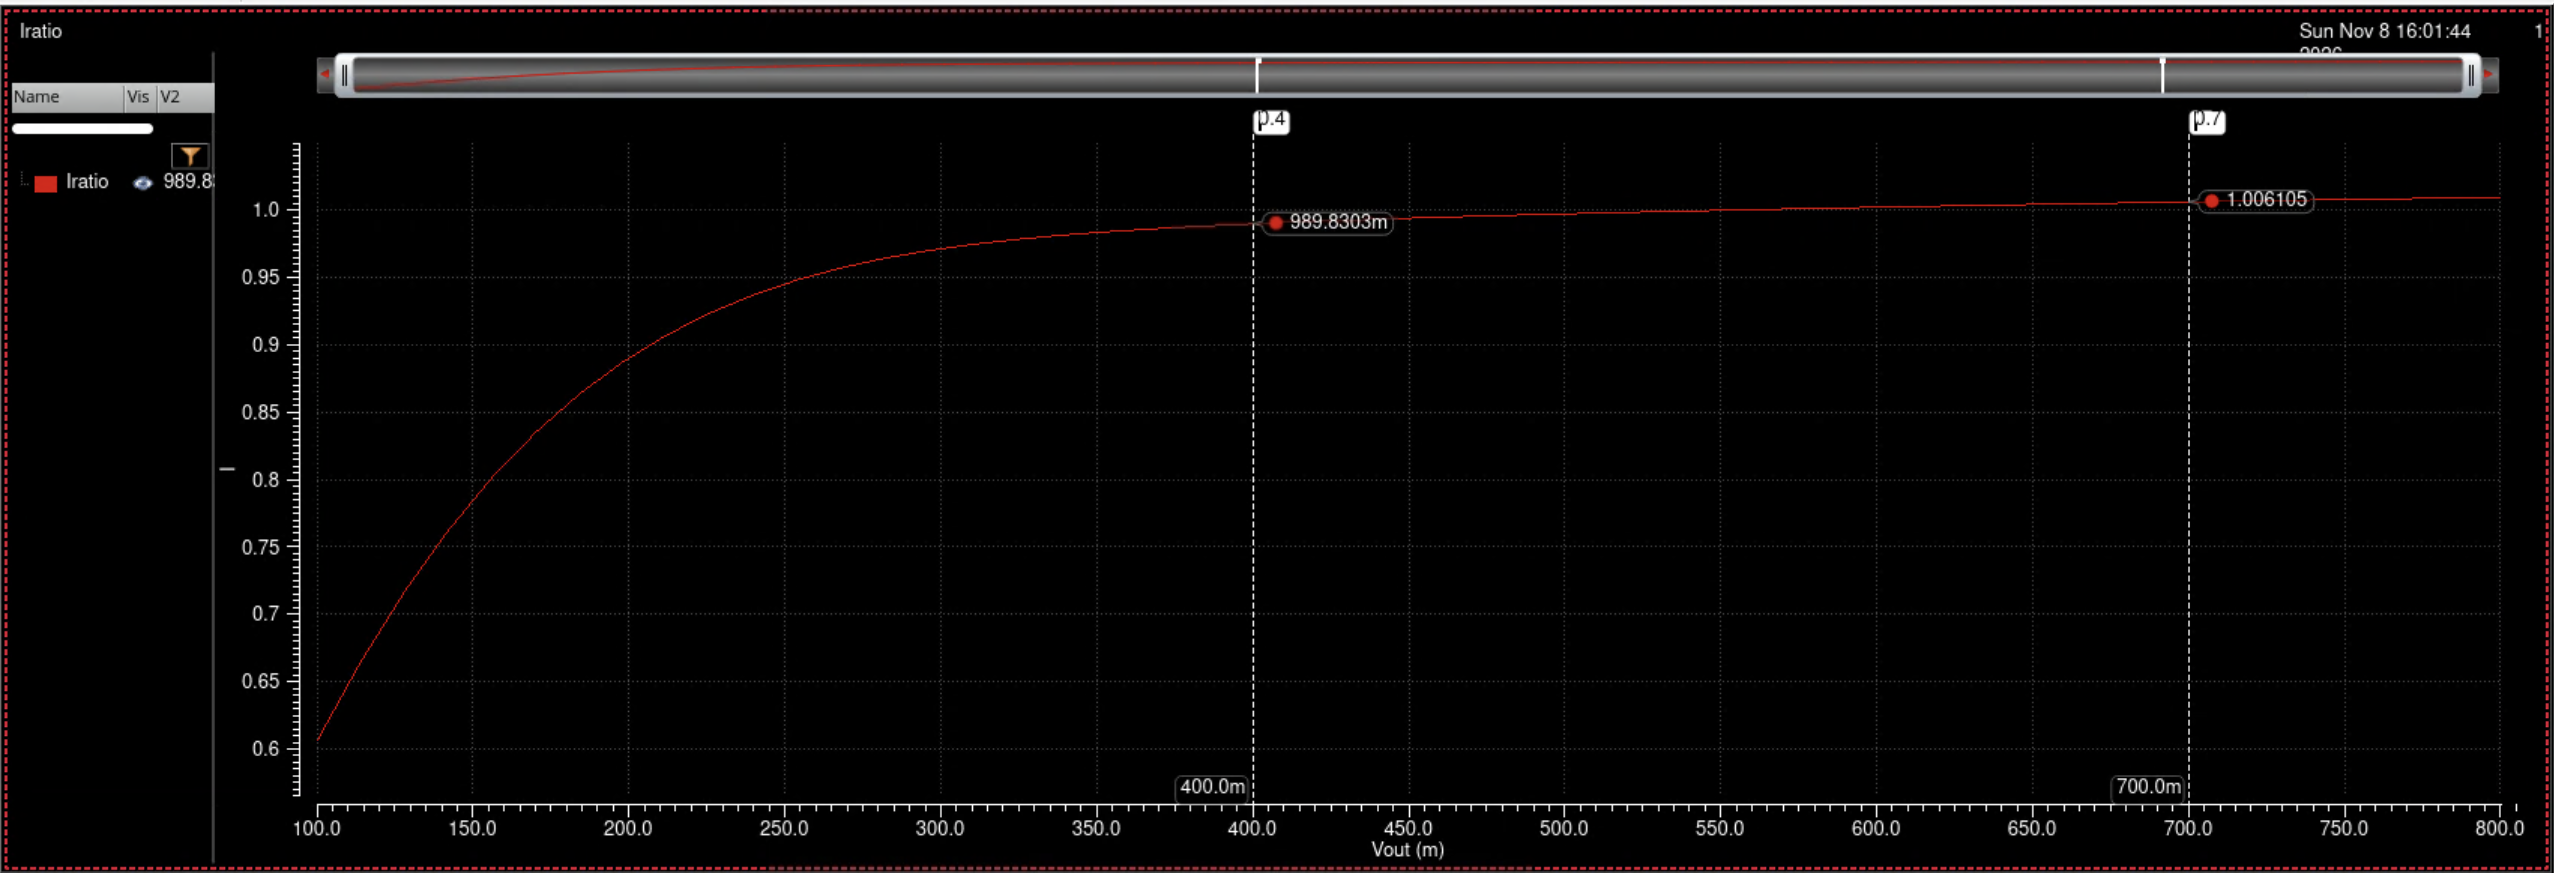
\includegraphics[width=0.9\textwidth,trim=600.0bp 301.5bp 4.5bp 50.0bp,clip]{P2_Iratio.png}
  \caption{Problem 2：$\ratio$ vs.\ $\Vout$（$V_b=0.72$\,V），下方為 0.4\,V 與 0.7\,V marker 區域放大。}
  \label{fig:p2ratio}
\end{figure}

曲線在約 0.3--0.35\,V 以下快速下降，對應 $M_4$ 離開飽和區（$\Vout<V_b-V_{TH4}\approx0.34$\,V）；
之上則非常平坦，並在 $\Vout\approx V_{GS1}\approx0.55$\,V 附近通過 1
（此時 $V_{DS4}=V_{DS3}$，$V_Y=V_X$，兩支路完全對稱）。

\subsection*{(c) 與 Problem 1 比較}

\begin{table}[H]
  \centering
  \caption{Mismatch 比較（皆為 $L=20$\,nm）}
  \label{tab:p2}
  \begin{tabular}{lccc}
    \toprule
                           & mismatch @ 0.4\,V   & mismatch @ 0.7\,V   & 等效 $\lambda$                     \\
    \midrule
    Problem 1 basic mirror & $-4.46\%$           & $+5.02\%$           & $\approx 0.36\ \mathrm{V^{-1}}$  \\
    Problem 2 cascode      & $-1.02\%$           & $+0.61\%$           & $\approx 0.042\ \mathrm{V^{-1}}$ \\
    \midrule
    改善倍數                   & $\approx 4.4\times$ & $\approx 8.2\times$ & $\approx 8.5\times$              \\
    \bottomrule
  \end{tabular}
\end{table}

Cascode 大幅降低了 mismatch。原因有二：
\begin{enumerate}\setlength{\itemsep}{0pt}
  \item 輸出阻抗提高：$R_{out}\approx g_{m4}r_{o4}r_{o2}$，比 basic mirror 的 $r_{o2}$ 大約 $g_m r_o$ 倍。
        $\Vout$ 的變化幾乎全落在 $M_4$ 上，$V_Y$ 只變化約 $\Delta\Vout/(g_{m4}r_{o4})$。
        改善約 8 倍，與 20\,nm 短通道元件不高的本質增益 $g_m r_o$ 相符。
  \item $M_1$、$M_2$ 的 $V_{DS}$ 被迫相等（$V_X\approx V_Y$），即使 $\lambda$ 很大也能精確複製電流。
\end{enumerate}
0.4\,V 的改善（4.4 倍）比 0.7\,V（8.2 倍）小，因為 0.4\,V 較接近 $M_4$ 的飽和邊界，
$M_4$ 的 $V_{DS}$ 只有約 0.22\,V，$g_{m4}r_{o4}$ 較小、曲線尚未完全變平。
這反映 cascode 的代價：提高輸出阻抗的同時，最低輸出電壓也從 Problem 1 的 $V_{DS,sat}\approx0.1$\,V
提高到約 $V_b-V_{TH}\approx0.34$\,V，輸出擺幅變小。

%=====================================================================
\section{Resistor-Biased Current Mirror with Ratio（Fig.~3）}

使用 Problem 1 的長通道元件（nFin $=2$、$L=240$\,nm），以電阻 $R$ 取代 $\Iref$，
$M_2$ 由 $m=4$ 個單位元件組成（CDF Multiplier $=4$，nFin 與 $L$ 不變）。

\begin{figure}[H]
  \centering
  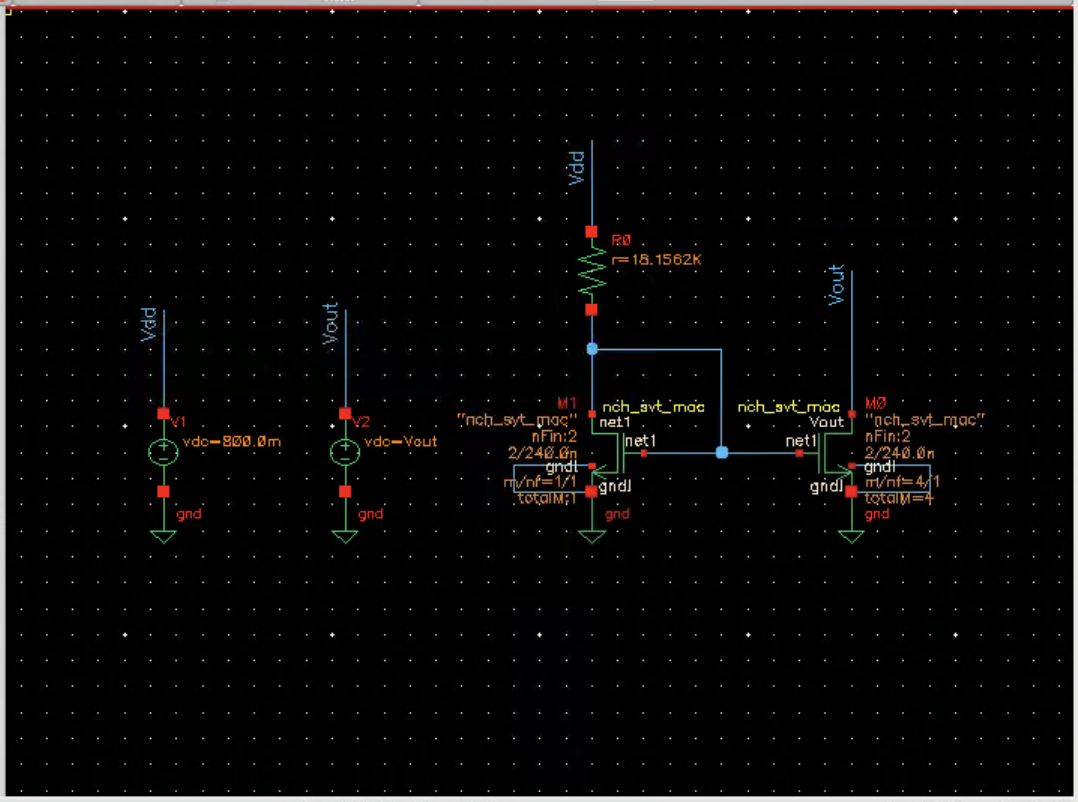
\includegraphics[width=0.85\textwidth,trim=58.0bp 117.0bp 41.5bp 64.0bp,clip]{P3_schematic.png}
  \caption{Problem 3 schematic（$R=18.1562$\,k$\Omega$；M0 為 $m/nf=4/1$，totalM $=4$）。}
  \label{fig:p3sch}
\end{figure}

\subsection*{(a) 選擇 $R$ 使 $\Iref\approx10\,\mu$A}
$M_1$ 為 diode-connected，閘極不汲取電流，故
\[
  \Iref=\frac{V_{DD}-V_{GS1}}{R}\quad\Rightarrow\quad R=\frac{0.8-V_{GS1}}{10\,\mu\mathrm{A}}.
\]
由 Problem 1 長通道結果（20\,$\mu$A 時 overdrive $\approx0.37$\,V），以平方律估計 10\,$\mu$A 時
overdrive $\approx0.37/\sqrt2\approx0.26$\,V，$V_{GS1}\approx0.62$\,V，$R\approx18$\,k$\Omega$。

精確值以 DC sweep 掃描 $R$（10--30\,k$\Omega$）決定（Fig.~\ref{fig:p3res}）：
$I=10\,\mu$A 對應 $R=18.16$\,k$\Omega$。
以此 $R$ 標註工作點（Fig.~\ref{fig:p3dc}）：$V_R=181.5$\,mV，$\Iref=9.999\,\mu$A，$V_{GS1}=617.8$\,mV，與估計相符。
（$\Iref$ 不受 $\Vout$ 影響，因為 $M_2$ 閘極不汲取電流。）

\begin{figure}[H]
  \centering
  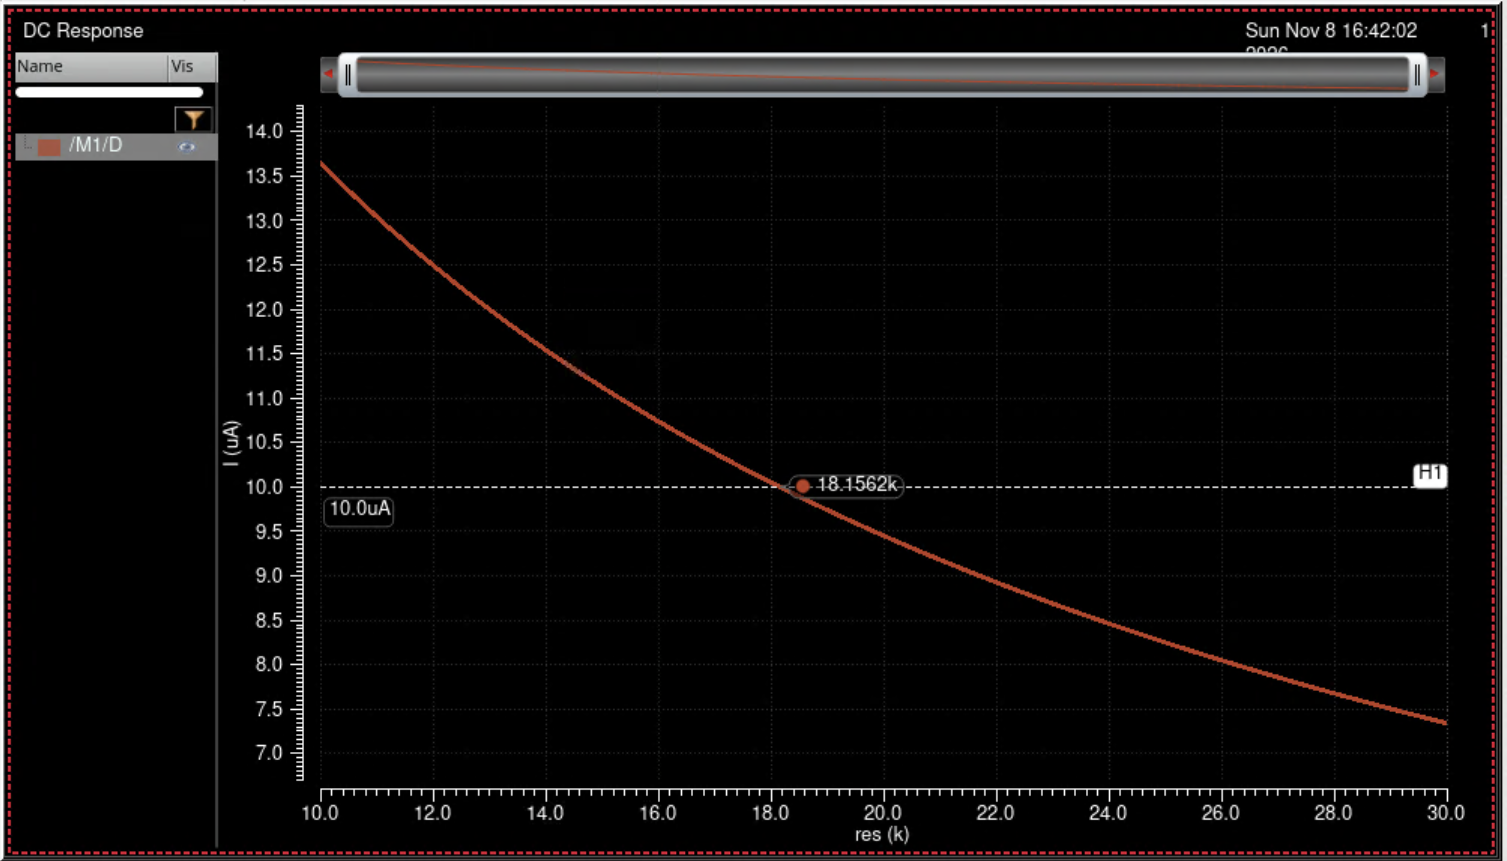
\includegraphics[width=0.8\textwidth]{P3_res.png}
  \caption{Problem 3：流過 $R$（$M_1$ drain）的電流 vs.\ $R$，水平 marker 為 10\,$\mu$A。}
  \label{fig:p3res}
\end{figure}

\begin{figure}[H]
  \centering
  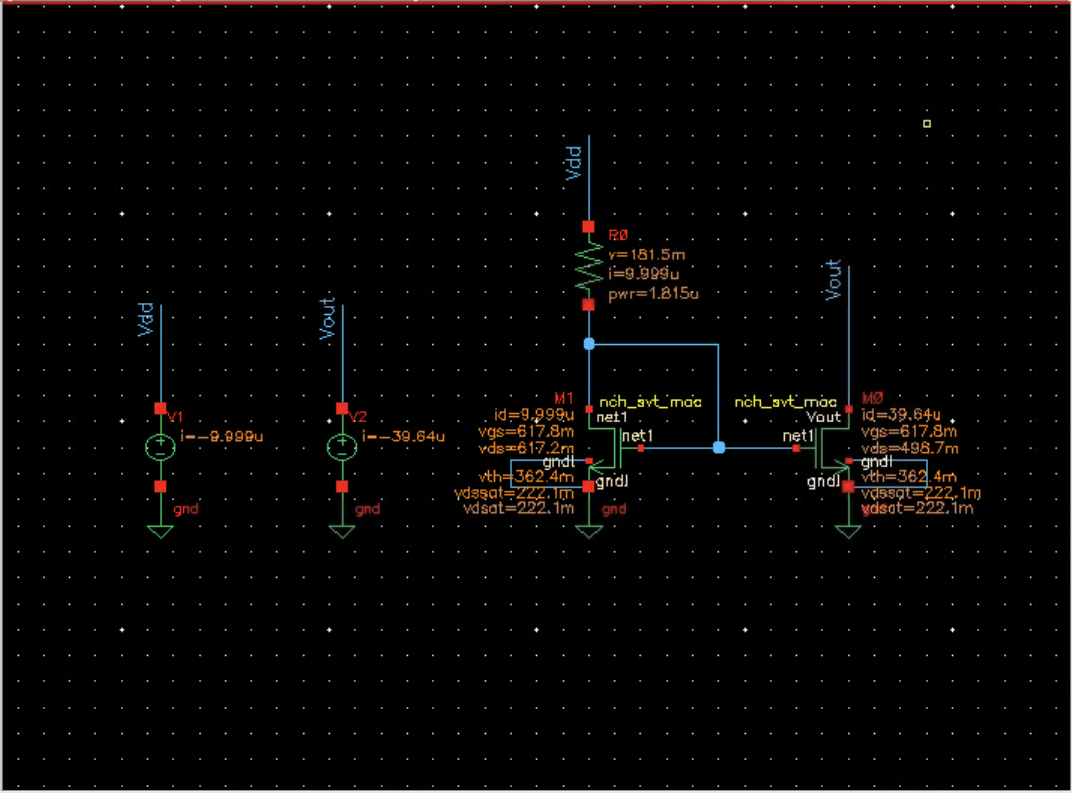
\includegraphics[width=0.85\textwidth,trim=56.5bp 115.0bp 33.5bp 47.5bp,clip]{P3_dcQ.png}
  \caption{Problem 3 DC operating point（$R=18.16$\,k$\Omega$，$\Vout=0.5$\,V）。}
  \label{fig:p3dc}
\end{figure}

由於 $V_{DD}-V_{GS1}$ 只有約 0.18\,V，$\Iref$ 對 $V_{DD}$ 與 $V_{TH}$ 的變動很敏感：
$V_{GS1}$ 或 $V_{DD}$ 偏移 18\,mV 即造成約 10\% 的電流變化。這是以電阻產生參考電流的缺點。

\subsection*{(b) $\Vout=V_{GS1}$ 時的 $\ratio$}

\begin{figure}[H]
  \centering
  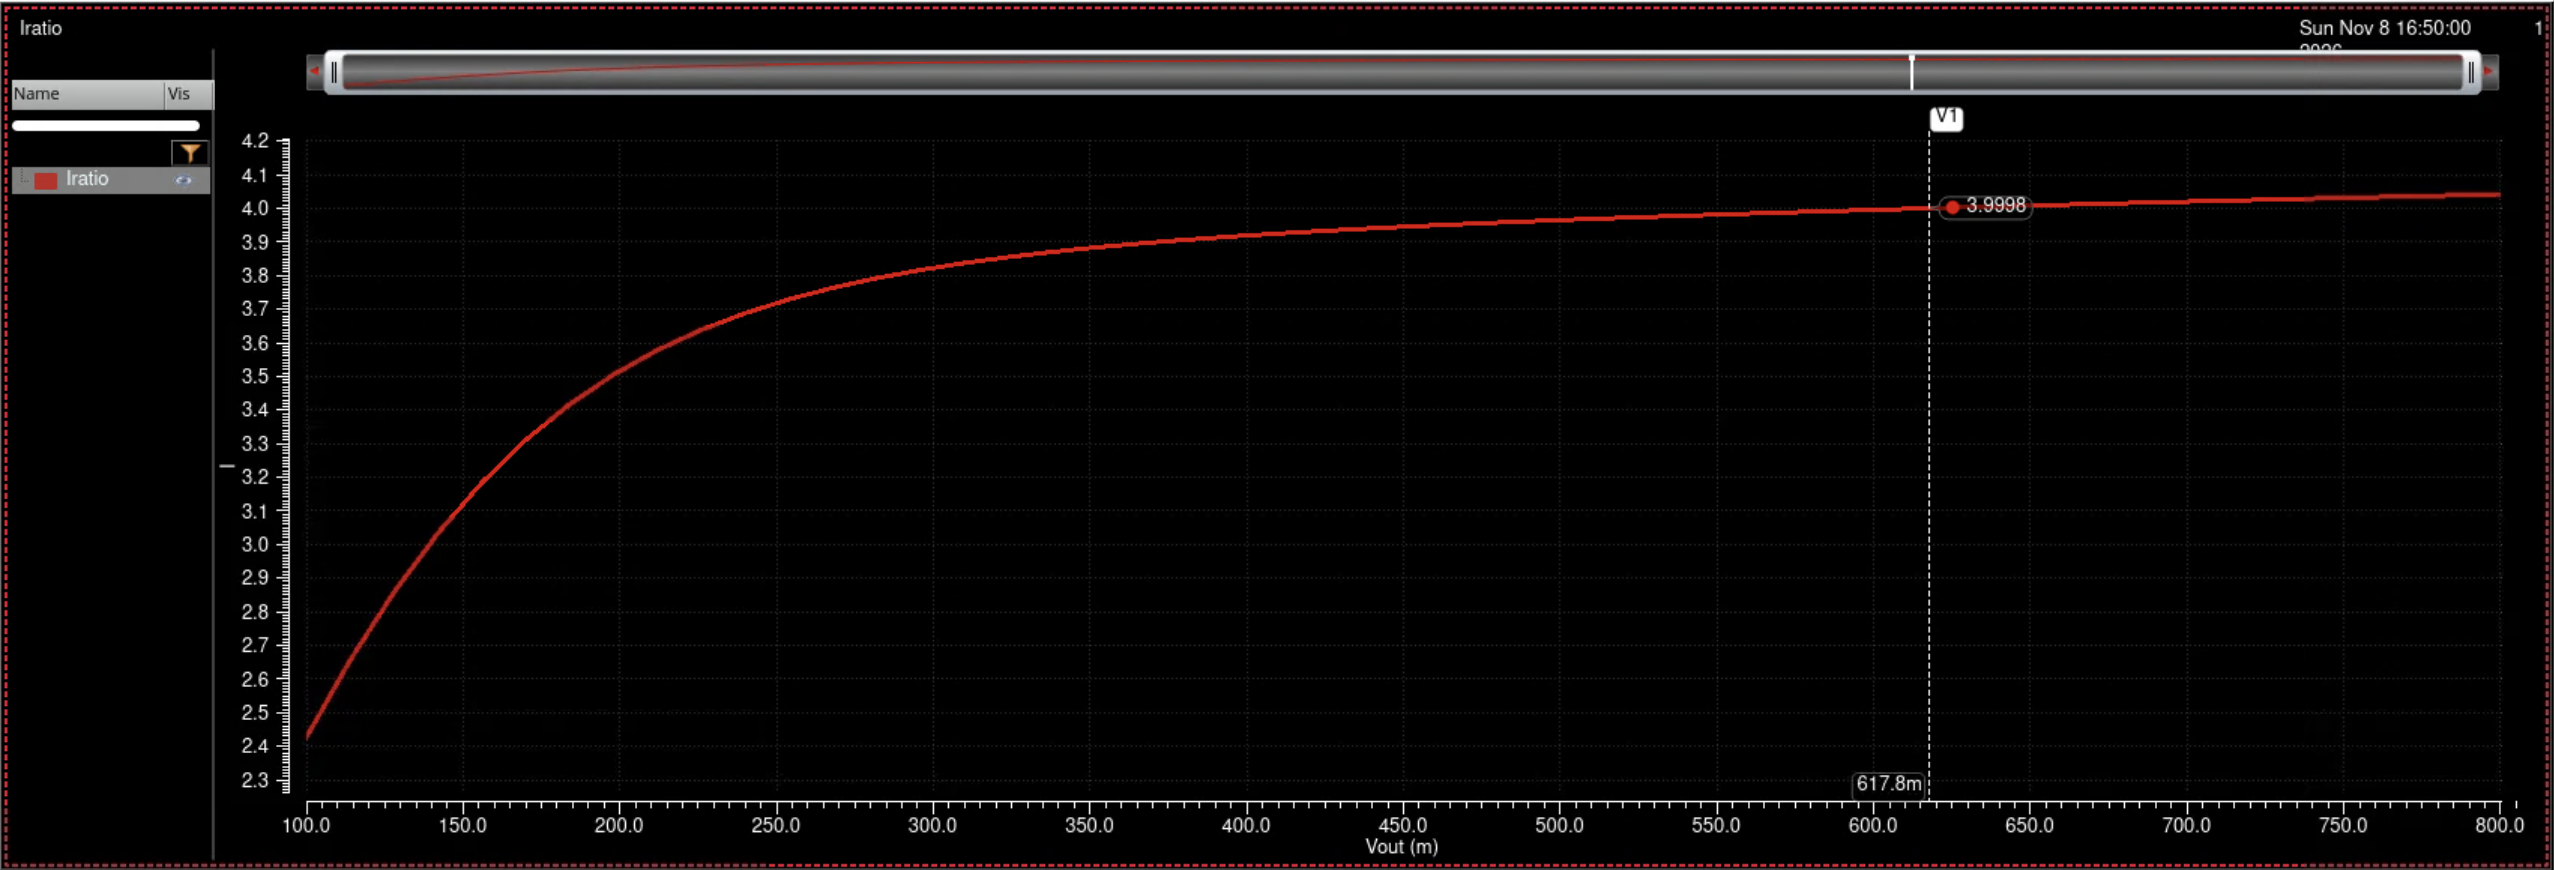
\includegraphics[width=\textwidth]{P3_Iratio.png}
  \\[3pt]
  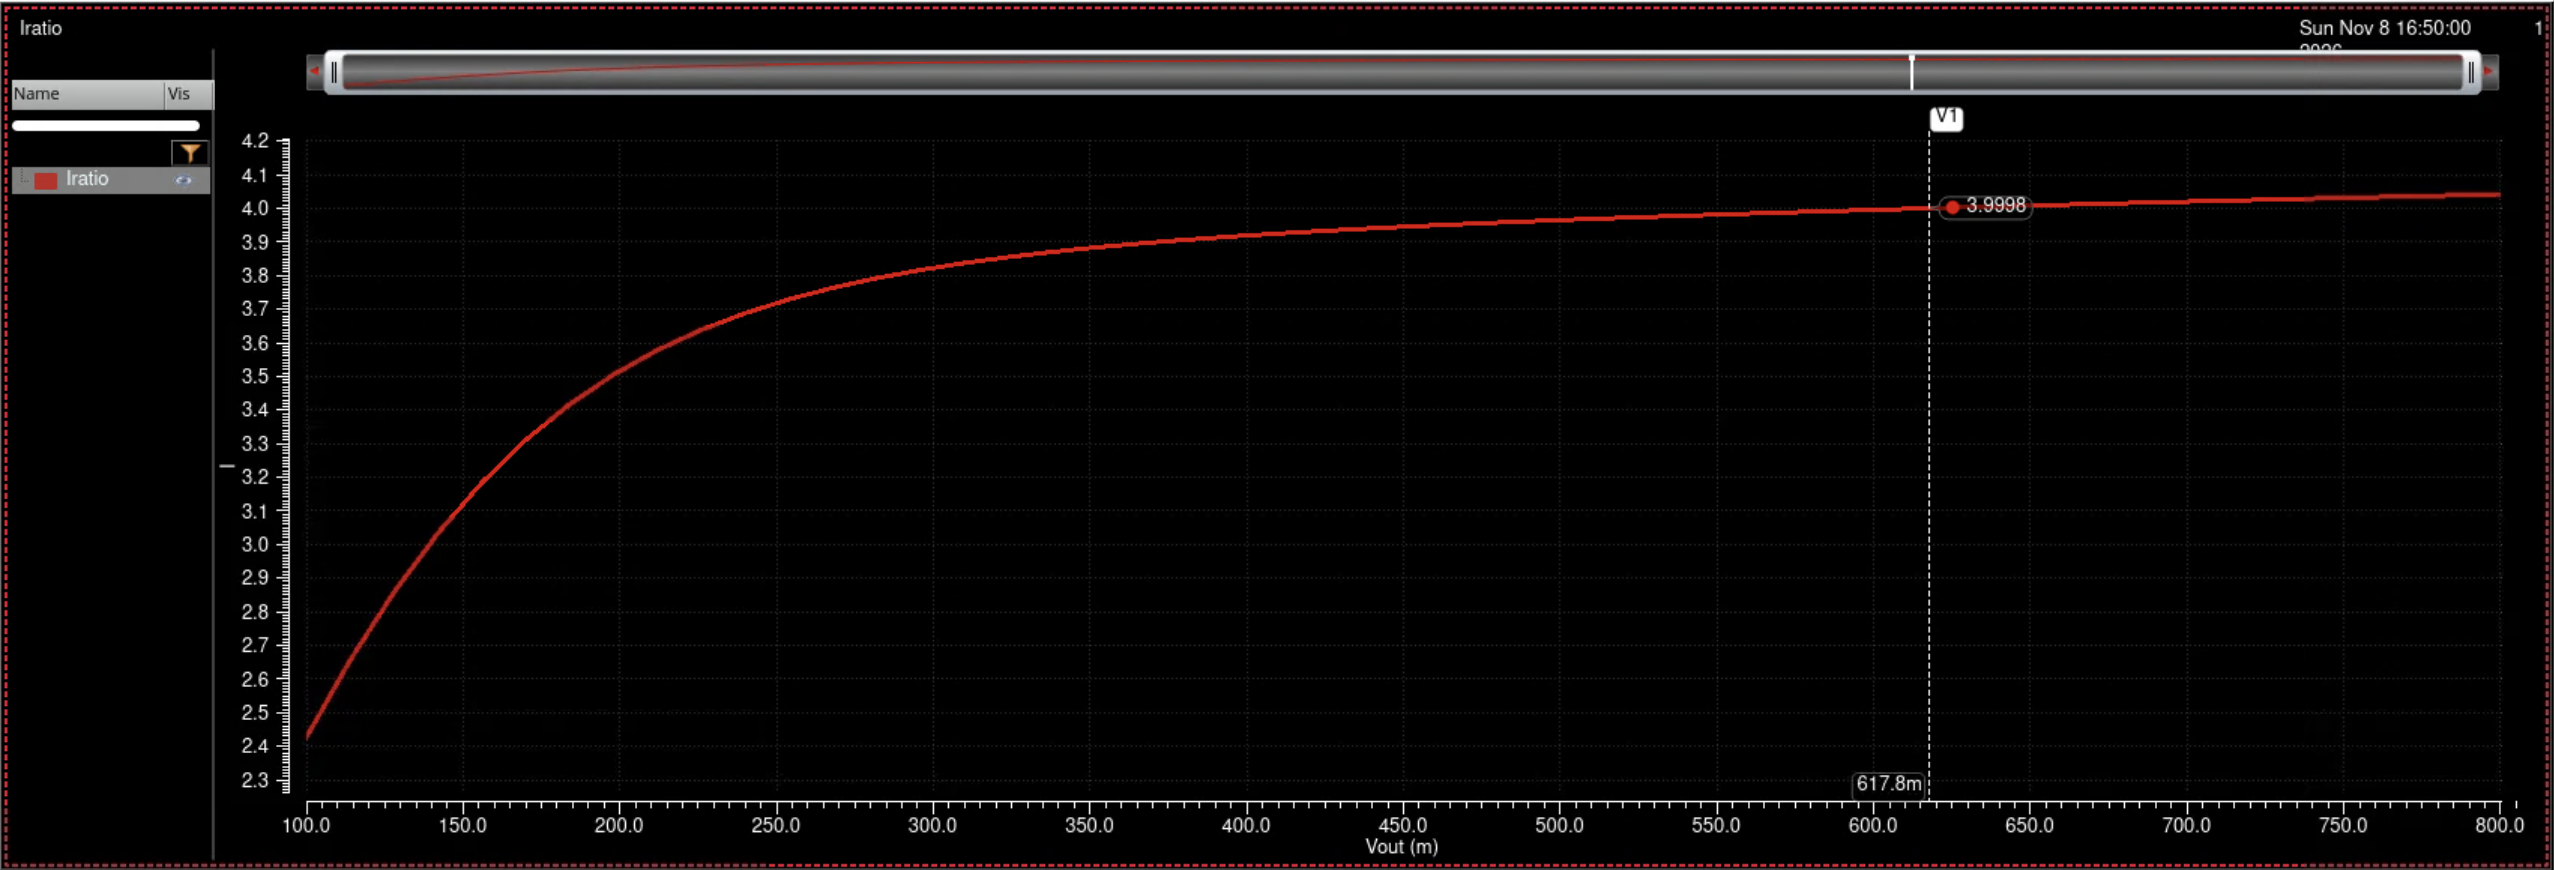
\includegraphics[width=0.9\textwidth,trim=750.0bp 305.0bp 4.5bp 50.0bp,clip]{P3_Iratio.png}
  \caption{Problem 3：$\ratio$ vs.\ $\Vout$，marker 位於 $\Vout=V_{GS1}=617.8$\,mV，下方為 marker 區域放大。}
  \label{fig:p3ratio}
\end{figure}

在 $\Vout=V_{GS1}=617.8$\,mV 時，$\ratio=\mathbf{3.9998\approx4}$，即 $\Iout\approx40\,\mu$A。
此時 $M_2$ 的 4 個單位元件與 $M_1$ 具有相同的 $V_{GS}$、$V_{DS}$ 與尺寸，各流 $\Iref$，
故 $\ratio=m=4$。偏離此點時比值因 channel-length modulation 而偏離 4
（例如 $\Vout=0.5$\,V 時 $\Iout=39.64\,\mu$A，比值 3.964，誤差約 $-0.9\%$）；
由於使用長通道元件，曲線在飽和區相當平坦。

\end{document}
